\chapter{Introduction} \label{cha:intro}
This chapter introduces some of the necessary background required for the rest of this thesis.  First, a general overview of the field of Visualization is provided with its benefits, drawbacks, and dangers for providing context to the rest of the work.  Second, a commonly used version of the visualization pipeline is introduced, elaborating on some of its relevant internal attributes.  The third section presents a small overview over interaction design and its requirements regarding the design of systems where it is essential to have a human-in-the-loop approach.  The last section reviews the literature and elaborates on the fundamentals of user evaluations that seek to answer the question whether novel visualization or interaction techniques are more effective than previous methods.

This chapter is not exhaustive by any means and the inclined reader searching for more detailed information is referred to a great selection of books, such as Preim and Bartz~\cite{preim2007visualization}, Preim and Botha~\cite{preim2013visual}, or Engel~\etal~\cite{engel2006real}.

\section{Visualization} \label{cha:intro:vis}
There have been many attempts at finding a universally accepted definition of \emph{Visualization}.  Card~\etal~suggested that Visualization is ``the use of computer-supported, interactive, visual representations of data to amplify cognition''~\cite{card1999readings}, while other definitions focus more on the interplay between generated imagery and the process of subjective visualization in each person [citation needed], or generalize the concept of visualization to non-visual phenomana as well [citation needed].  The commonality between these defintions is the focus on a human observer, the fact that a visualization is created for and by a human.  Furthermore, the field of visualization was started as, and continues to be, a reaction to the data explosion occurring in other fields~\cite{lorensen2004death}.

One distinction, the separation between \emph{explorational} and \emph{presentational} use cases was put forward, among others, by van Wijk~\cite{van2005value}.  This is addressed and elaborated in a later chapter (Chapter~\ref{cha:contributions}) and forms the basis of the contributions in this thesis.  At the heart is the realization that visualization can be achieved for different audiences and must adapt accordingly.

Card~\etal~\cite{card1999readings} and others often separate the field of visualization into at least three categories, \emph{Scientific Visualization}, \emph{Information Visualization}, and \emph{Visual Analytics}.

\paragraph{Scientific Visualization} is characterized by the use of data sources with an inherent physical component.  Data traditionally attributed to Scientific Visualization comes in the form of, for example, simulations or datasets in which the spatial relationship is trivially given.

\paragraph{Information Visualization} usually deals with abstract data that does not possess an innate spatial component.  Techniques from this part are typically high-dimensional and multi-variate.

\paragraph{Visual Analytics} places heavier focus on the analytical reasoning and the interaction modes in order to produce insight into the data rather than the source of the data itself.

Tory~\etal~\cite{tory2002model} pointed out that the required use of words such as ``usually'', ``typically'', or ``traditionally'' hints at a problem with this type of classification.  For once, it is not always possible to delineate differences between the categories even in the most trivial applications.  More complicated applications almost always use reseach from two or all three of these categories, increasing the difficult for a separation.  In their work, Tory~\etal~provide a more nuanced \emph{model-based taxonomy} that is based on the model of the data rather than the data itself.  Rather than using a taxonomy that is based on the description of the data, they propose a taxonomy that is based on the way the data is used inside the visualization system and differentiates between \emph{continous} and \emph{discrete} data, regardless of whether the data itself is abstract or spatial.  This lack of separation between the categories is used in this thesis as they are used to solve the same kinds of problems, displaying data to a human to facilitate insight, utilizing different tools and ``at this level there is much more they share than what separates them''~\cite{van2005value}.

\subsection{Benefits} \label{cha:intro:vis:benefits}
As mentioned in the previous chapter, humans are exceptionally well evolved to interpret the information contained in images.  This is exemplified by the popular quote that ``a picture is worth a thousand words'', meaning that it is significantly easier for humans to ingest information visually rather than through textual description.  Throughout many psychological studies [citation needed] it has been shown that there are two classes of problems.  On the one hand, there are problems that can be solved more efficiently by computers, such as searching large databases and algorithms that typically operate on a map-and-reduce scheme.  On the other hand, there are problems solved better by humans, such as pattern recognition, hypothesis forming, and others [citation needed?].  Visualization, being placed on the boundary between these two problems, can utilize the respective strengths of both computers and humans through a close integration.

\subsection{Limitations} \label{cha:intro:vis:limitations}
One of the important limiting factors influencing each visualization is its subjectiveness.  According to van Wijk, the benefit of using a visualization depends on ```the specification [$\cdots$], the perceptual skills of the observer, and the a priori knowledge of the observer''~\cite{van2005value}.  This is yet another reason why close collaboration between the visualization designer and the domain expert is of fundamental importance, as the design process has to take the experts knowledge into account.  Lorensen elaborated on the potential problems for the visualization community if this collaboration does not occur~\cite{lorensen2004death}.  Another direct consequence of this subjectiveness is that the reproducibility of a visualization is limited to similar consumers.  A visualization system that is designed for experts in a field is totally useless when the same data should be explained to a general public.  

Another aspect of the a priori knowledge that is often overlooked is a dependence on cultural background.  Whereas knowledge-based prior information can be easily assessed, it is much harded to assess cultural bisases.  Some of these cultural differences can be benign, such as the Western tendency to associate movement across a red-green color scale with an increasing value, whereas East Asian cultures would associcate this with a decreasing value, due to the flipped association between the red and green colors.  Other differences can be seen in Figure~\ref{fig:intro:vis:lego}, which displays characters from eight popular cartoon series built from Lego blocks and can be seen as a form of visualization.  Viewed in a culture that is completely unfamiliar with these characters, however, it becomes easy to see that this visualization will be unable to produce any meaningful results.

\begin{figure}
  \centering
  \fbox{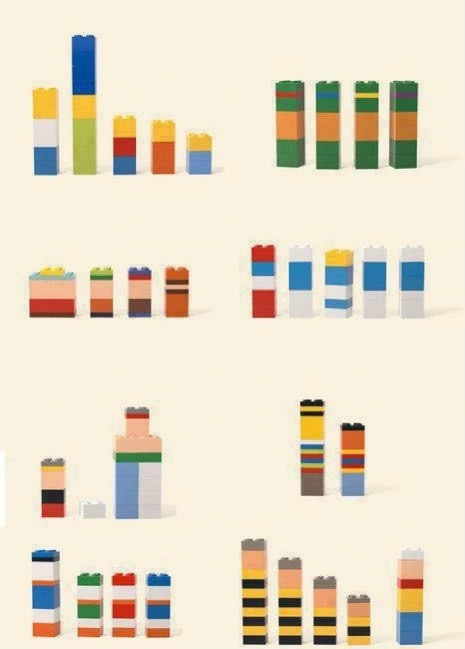
\includegraphics[width=\textwidth]{figures/intro/lego.jpg}}
  \caption{A collection of advertisement images representing cartoon characters. With the required cultural background, deciphering these visualizations is impossible. Image copyright by Lego. Reprinted with permission.}
  \label{fig:intro:vis:lego}
\end{figure}

\subsection{Dangers} \label{cha:intro:vis:dangers}
Besides the immense benefits that visualization can provide for supporting data interpretation and hypothesis testing, there are also aspects where the misuse of visualization can be dangerous to the knowledge increase.  One obvious aspect that is outside the scope of this work is the use of visualization to deliberately mislead the audience.  Even without a deliberate attempt, there are many pitfalls that need to be considered when designing a visualization.  Another danger of the use of visualization is exemplified in the quote from van Wijk saying that ``visualization should not be used to verify the final truth, but rather to inspire to new hypotheses, to be checked afterwards''.  Verifying truths, rather than inspiring hypotheses cna easily lead to confirmation biases that might lead experts to draw faulty conclusions.  Naturally, this danger can only occur in the initial exploration stages of a visualization and can be mitigated when a visualization system is matured and applied to many of the same types of datasets; nevertheless, it is an important aspect to consider during the design process.  The remaining dangers fall into two categories, \emph{showing incorrect information} and \emph{showing information incorrectly}. The first category can occur if visualization designers do not stay true to the data of the expert by, for example, applying smoothing to inherently concrete data sets, not handling outliers correctly in a filtering operation, or not considering missing data in real world datasets.  For the domain expert it becomes increasingly difficult to differentiate missing data from outliers in, for example, a simulation, thus eroding the expert's trust in a visualization system.  In the second category, color maps play a huge role.  Using ill-suited color maps it is trivially possible to highlight or hide structures in the data without informing the expert.  One example if this is the continued use of the rainbow color map in science publications even though it has been shown to be inferior to other color maps~\cite{borland2007rainbow}.



\section{Visualization Pipeline} \label{cha:intro:vp}
\begin{figure}
  \centering
  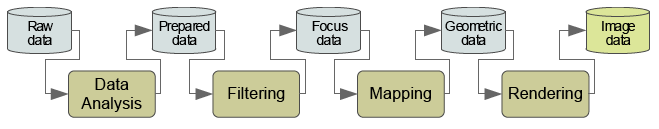
\includegraphics[width=\textwidth]{figures/intro/pipeline.png}
  \caption{One common version of the visualization pipeline as described by Dos Santos and Brodlie. The raw data is transformed multiple steps until an image is generated that can be used by the user to gain insight.  The ability for the user to control each part of the visualization pipeline is at the heart of the human-in-the-loop methodology.}
  \label{fig:intro:vp}
\end{figure}

Figure~\ref{fig:intro:vp} shows a schematic overview of the workflow employed by visualization techniques.  All visualization research attempts to improve one or more of these stages in the pipeline.  The pipeline used was first described by Haber and McNabb~\cite{haber1990visualization} and later extended by Dos Santos and Brodlie~\cite{dos2004gaining} and consists of four transformations that are successively applied to the incoming data.  For a complete description of the visualization pipeline at its variations, we refer to the two original works or by a survey about the development of the visualization pipeline by Moreland~\cite{moreland2013survey}.

One important aspect for the design of visualization application systems, that was not fully accounted for in the original visualization pipeline, is the feedback from the user into the various transformation stages.  While it was always possible to change the parameters of the \emph{Rendering} or \emph{Mapping} stages by, for example, changing the camera position, or changing the color attributes of the Abstract Visualization Objects of the \emph{Geometric Data}, the focus of interactivity for the other steps of the pipeline was introduced later with increasing distance from the user.  One of the last feedback loops, Computational Steering, was described by Mulder~\etal~\cite{mulder1999survey}, where the visualization user is able to directly influence the gathering of the \emph{Raw Data} with minimal delay.  Closing this feedback loop leads to the biggest gain in insight as the user can, in the example of simulations, directly understand the influence of parameter changes and can thus gain a deeper understanding of the origin of the data.

\begin{figure}
  \centering
  \fbox{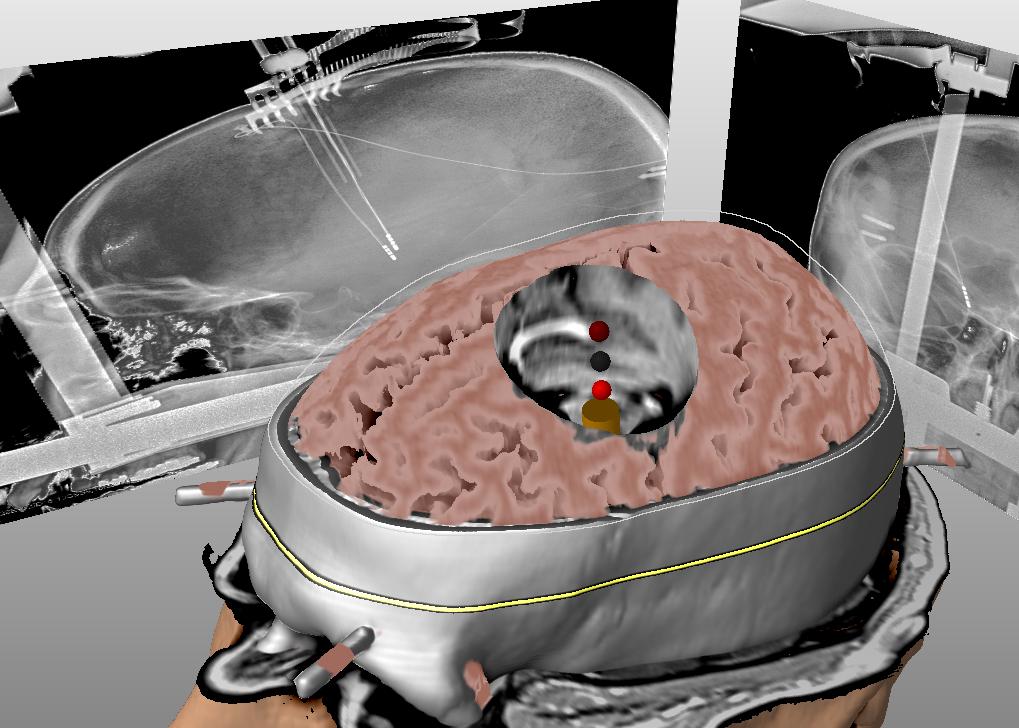
\includegraphics[width=0.5\textwidth]{figures/intro/magicmirror.png}}
  \caption{One example of a multiview visualization, a \emph{Magic Mirror}, where X-ray scans of a patients are shown projected to the sides of a combined volumetric rendering.}
  \label{fig:intro:mm}
\end{figure}

Another important aspect of the visualization pipeline that is hidden from the pipeline depicted in the figure is the possibility of pipeline branching.  Multiview visualization systems provide multiple simultaneous views on different aspects of the data.  One example of these techniques is a magic mirror~\cite{konig1999multiple} as shown in Figure~\ref{fig:intro:mm} that presents different aspects of the underlying data are shown projected to the sides of a surrounding cube.  In a multiview systems, separate branches of the pipeline handle these different views that are ultimately merged in the \emph{Rendering} step.  There exists a large amount of research on techniques dealing with multiview systems, such as brushing or linking~\cite{tory2003mental}.

\subsection{Data Acquisition} \label{cha:intro:vp:da}

\subsubsection{Data Types} \label{cha:intro:vp:da:types}
Different data types

\paragraph{X-Ray. }
\paragraph{Computer Tomography. }
\paragraph{Magnetic Resonance Imaging. }
\paragraph{Simulations. }

\subsubsection{Grids} \label{cha:intro:vp:da:grids}
\paragraph{Cartesian}

\paragraph{Spherical}

\subsection{Direct Volume Rendering} \label{cha:intro:vp:dvr}
\begin{itemize}
  \item Emission/absorption \cite{sabella1988rendering}
  \item Volume rendering integral \cite{max1995optical}
  \item Other techniques
  \begin{itemize}
    \item MIP / MIDA / isosurface
    \item Object-order: texture slicing \cite{westermann1998efficiently}, splatting \cite{westover1990footprint}
    \item Image-order: volume raycasting \cite{levoy1988display, drebin1988volume,sabella1988rendering} speedup: \cite{kruger2003acceleration} single pass rendering \cite{hadwiger2005real, stegmaier2005simple}
  \end{itemize}
  \item Raycasting v raytracing
\end{itemize}

\section{Human-in-the-Loop} \label{cha:intro:hitl}
\begin{itemize}
  \item Combination of automated systems and human-in-the-loop; Shows importance of domain expert integration
  \begin{itemize}
    \item Interaction design
    \item \cite{munzner2014visualization} \cite{van2005value} -> Shows importance of domain expert integration
  \end{itemize}
\end{itemize}
